%%%%%%%%%%%%%%%%%%%%%%%%%%%%%%%%%%%%%%%%%%%%%%%%%%%%%%%%%%%%
%%  This Beamer template was created by Cameron Bracken.
%%  Anyone can freely use or modify it for any purpose
%%  without attribution.
%%
%%  Last Modified: January 9, 2009
%%

\documentclass[xcolor=x11names,compress]{beamer}

%% General document %%%%%%%%%%%%%%%%%%%%%%%%%%%%%%%%%%
\usepackage{graphicx}
\usepackage{tikz}
\usetikzlibrary{decorations.fractals}
%%%%%%%%%%%%%%%%%%%%%%%%%%%%%%%%%%%%%%%%%%%%%%%%%%%%%%
%%%%%%%%%%%%%%%%%%%%%%%%%%%%%%%%%%%%%%%%%%%%%%%%%%%%%%
\usepackage{caption} % removing prefix from figure caption in LaTeX
\usepackage{multirow}
\usepackage{multicol}
\usepackage{systeme}
%%%%%%%%%%%%%%%%%%%%%%%%%%%%%%%%%%%%%%%%%%%%%%%%%%%%%%
% Font size
%%%%%%%%%%%%%%%%%%%%%%%%%%%%%%%%%%%%%%%%%%%%%%%%%%%%%%
\usepackage{lipsum}
\newcommand\Fontvi{\fontsize{6}{7.2}\selectfont}

%% Beamer Layout %%%%%%%%%%%%%%%%%%%%%%%%%%%%%%%%%%
\useoutertheme[subsection=false,shadow]{miniframes}
\useinnertheme{default}
\usefonttheme{serif}
\usepackage{palatino}
\usepackage{wrapfig}
\usepackage{float}
\usepackage{verbatim}

\setbeamerfont{title like}{shape=\scshape}
\setbeamerfont{frametitle}{shape=\scshape}

\setbeamercolor*{lower separation line head}{bg=DeepSkyBlue4} 
\setbeamercolor*{normal text}{fg=black,bg=white} 
\setbeamercolor*{alerted text}{fg=red} 
\setbeamercolor*{example text}{fg=black} 
\setbeamercolor*{structure}{fg=black} 
 
\setbeamercolor*{palette tertiary}{fg=black,bg=black!10} 
\setbeamercolor*{palette quaternary}{fg=black,bg=black!10} 

\renewcommand{\(}{\begin{columns}}
\renewcommand{\)}{\end{columns}}
\newcommand{\<}[1]{\begin{column}{#1}}
\renewcommand{\>}{\end{column}}

\newcommand\xput[2][0.1]{%
    \rule{#1\linewidth}{0pt}\makebox[0pt][c]{#2}\hfill}

%%%%%%%%%%%%%%%%%%%%%%%%%%%%%%%%%%%%%%%%%%%%%%%%%%%%%%
% Graphs path to the Picture Folder
%%%%%%%%%%%%%%%%%%%%%%%%%%%%%%%%%%%%%%%%%%%%%%%%%%%%%%
%\graphicspath{/home/henry/Desktop/UTEP_Proposal_Thesis/PhD_Thesis/Pictures}
\graphicspath{{Pictures/}{Data/}} % Two folders Picture and Data    
    
%%%%%%%%%%%%%%%%%%%%%%%%%%%%%%%%%%%%%%%%%%%%%%%%%%%%%%
%Graphs
%%%%%%%%%%%%%%%%%%%%%%%%%%%%%%%%%%%%%%%%%%%%%%%%%%%%%%
\usepackage{graphics}
\usepackage{graphicx}
\usepackage{texdraw}
\usepackage{color}
\usepackage{subfigure} 
\usepackage{epsfig}
%\usepackage{pst-grad} % For gradients
%\usepackage{pst-plot} % For axes
%\usepackage{movie15}
\usepackage{booktabs}
\usepackage{animate}
\usepackage{wrapfig}
\usepackage[font={small}]{caption}    

\usepackage{lipsum}
\setbeamercolor*{block body}{bg=white,fg=black}
\setbeamercolor*{block title}{fg=white,bg=blue}
\setbeamerfont{block title}{size=\Large}
    
%%%%%%%%%%%%%%%%%%%%%%%%%%%%%%%%%%%%%%%%%%%%%%%%%%
\begin{document}
%%%%%%%%%%%%%%%%%%%%%%%%%%%%%%%%%%%%%%%%%%%%%%%%%%%%%%
%%%%%%%%%%%%%%%%%%%%%%%%%%%%%%%%%%%%%%%%%%%%%%%%%%%%%%
\section{}
\begin{frame}
\title{How to use BLAS and LAPACK\\ with a\\C Languages Programming}
%\subtitle{Las matem\'aticas que no est\'an escritas en \LaTeX\@ no son matem\'aticas serias.\\
%\LaTeX\@ una herramienta para procesar textos utilizando Software Libre}

\author{
	Henry R. Moncada\\
	{\it University of Texas at El Paso}\\
}
\date{
	\begin{tikzpicture}[decoration=Koch curve type 2] 
		\draw[DeepSkyBlue4] decorate{ decorate{ decorate{ (0,0) -- (3,0) }}}; 
	\end{tikzpicture}  
	\\
	\vspace{.5cm}
	\today
}
\titlepage
\end{frame}
%%%%%%%%%%%%%%%%%%%%%%%%%%%%%%%%%%%%%%%%%%%%%%%%%%%%%%
%%%%%%%%%%%%%%%%%%%%%%%%%%%%%%%%%%%%%%%%%%%%%%%%%%%%%%
\begin{frame}{Contenido}
\tableofcontents
\end{frame}
%%%%%%%%%%%%%%%%%%%%%%%%%%%%%%%%%%%%%%%%%%%%%%%%%%%%%%
%%%%%%%%%%%%%%%%%%%%%%%%%%%%%%%%%%%%%%%%%%%%%%%%%%%%%
\section{\scshape Linear Algebra}
\begin{frame}[fragile]{Linear Algebra}
The purpose of this presentation is to show you how to use \textbf{BLAS\;/LAPACK} functions in your own C/C++ or Fortran code.
For this, Let us explain how to solves a system of linear equations.  
%https://dynamithead.wordpress.com/2012/06/30/introduction-to-how-to-call-lapack-from-a-cc-program-example-solving-a-system-of-linear-equations/
\begin{eqnarray*}
 x_1 + 2 x_2 + 3 x_3 & = & -4 \\
 2 x_1 + 3 x_2 + 4 x_3 & = & -1 \\
 3 x_1 + 4 x_2 + x_3 & = & -2 
\end{eqnarray*}
Solving this system of linear equations, we get the following solutions:
\[(x_1,x_2,x_3) = (11,-9,1)\]
% \[
% \systeme*{x_1=2r + s -t,x_2= r, x_3=-2s +2t, x_4=s, x_5=t}
% \]
\end{frame}

%%%%%%%%%%%%%%%%%%%%%%%%%%%%%%%%%%%%%%%%%%%%%%%%%%%%%%
%%%%%%%%%%%%%%%%%%%%%%%%%%%%%%%%%%%%%%%%%%%%%%%%%%%%%
\section{}
\begin{frame}[fragile]{Linear Algebra}
Rewriten the system of linear equations in a matrix/array form
\[\left[\begin{array}{ccc}
 1 & 2 & 3 \\
 2 & 3 & 4\\        
 3 & 4 & 1 
\end{array}\right]
\left[\begin{array}{c}
x_1\\
x_2\\
x_3 
\end{array}\right]
= \left[\begin{array}{c}
-4\\
-1\\
-2 
\end{array}\right]\]
We can represented the system using coefficients:
\begin{itemize}
\item $A$ is coefficient matrix,
\item $b$ is the vector containing the right sides of equations,
\item $x$ is the vector containing the solutions of equations.
\end{itemize}

\begin{equation*}
 A\;x = b
\end{equation*}
\end{frame}
%%%%%%%%%%%%%%%%%%%%%%%%%%%%%%%%%%%%%%%%%%%%%%%%%%%%%%
%%%%%%%%%%%%%%%%%%%%%%%%%%%%%%%%%%%%%%%%%%%%%%%%%%%%%
\section{}
\begin{frame}[fragile]{Linear Algebra}
\begin{equation*}
 A\;x = b 
\end{equation*}
The square matrix $A$ is invertible, if there exists a matrix $A^{-1}$ such that
\begin{equation*}
A^{-1}\;A = A\;A^{-1} = I
\end{equation*}
where $I$ is the identity matrix. 
\begin{equation*}
\mbox{If } \exists \; A^{-1} \;\; \Leftrightarrow \;\; det(A) \neq 0
\end{equation*}
The solution of the system of linear equations can be solved as following
\begin{eqnarray*}
 Ax & = & b \\
 A^{-1}A x & = & A^{-1}\;b\\
 x & = & A^{-1}\;b\Rightarrow x = A\backslash b
\end{eqnarray*}
\end{frame}

%%%%%%%%%%%%%%%%%%%%%%%%%%%%%%%%%%%%%%%%%%%%%%%%%%%%%%
%%%%%%%%%%%%%%%%%%%%%%%%%%%%%%%%%%%%%%%%%%%%%%%%%%%%%
\section{\scshape Matlab and Intel Math Kernel Library (MKL)}
\begin{frame}[fragile]{Matlab and Intel Math Kernel Library (MKL)}
\begin{scriptsize}
\begin{itemize}
\item Intel MKL is a library of optimized math routines for science, engineering, and financial applications.
\item Core math functions include BLAS, LAPACK, ScaLAPACK, sparse solvers, fast Fourier transforms, and vector math. 
\item The routines in MKL are hand-optimized specifically for Intel processors.
\item Utilizes standard C and Fortran APIs for compatibility with BLAS, LAPACK and FFTW functions from other math libraries.
\item It is available with both free community-supported and paid support licenses.
\item MATLAB uses the Intel Math Kernel Library (MKL) behind the scenes to perform many linear algebra operations. 
\end{itemize}
What version of the MKL was being used by MATLAB. Let's ask MATLAB
\end{scriptsize}
\begin{tiny}
\begin{verbatim}
 >> version -lapack
ans =
Intel(R) Math Kernel Library Version 10.3.5 Product Build 20110720 for
Intel(R) 64 architecture applications

>> version -blas
ans =
Intel(R) Math Kernel Library Version 10.3.5 Product Build 20110720 for
Intel(R) 64 architecture applications
\end{verbatim}
\end{tiny}
\end{frame}
%%%%%%%%%%%%%%%%%%%%%%%%%%%%%%%%%%%%%%%%%%%%%%%%%%%%%%
%%%%%%%%%%%%%%%%%%%%%%%%%%%%%%%%%%%%%%%%%%%%%%%%%%%%%
\section{\scshape BLAS,and LAPACK}%, and ATLAS}
\begin{frame}[fragile]{BLAS, and LAPACK}%, and ATLAS}
%http://stackoverflow.com/questions/17858104/what-is-the-relation-between-blas-lapack-and-atlas
\begin{scriptsize}
\begin{itemize}
\item \textbf{BLAS (Basic Linear Algebra Subprograms)} is a collection of low-level matrix and vector arithmetic operations, for performing common linear algebra operations such as vector addition, scalar multiplication, dot products, linear combinations, and matrix multiplication.
		
\item \textbf{LAPACK (Linear Algebra Package)} is a collection of higher-level linear algebra operations. It provides routines for solving systems of linear equations such as matrix factorizations (LU, LLt, QR, SVD, Schur, etc), linear least squares, eigenvalue problems, and singular value decomposition. LAPACK is built on top of the BLAS; many users of LAPACK only use the LAPACK interfaces and never need to be aware of the BLAS at all. LAPACK is generally compiled separately from the BLAS, and can use whatever highly-optimized BLAS implementation you have available.
%\item\textbf{ ATLAS (Automatically Tuned Linear Algebra Software)} is a software library for linear algebra. It provides a mature open source implementation of BLAS. The ATLAS  project is an ongoing research effort focusing on applying empirical techniques in order to provide portable performance. At present, it provides a portable and efficient BLAS implementation, as well as a few routines from LAPACK.
\end{itemize}
\end{scriptsize}
\end{frame}
%%%%%%%%%%%%%%%%%%%%%%%%%%%%%%%%%%%%%%%%%%%%%%%%%%%%%%
%%%%%%%%%%%%%%%%%%%%%%%%%%%%%%%%%%%%%%%%%%%%%%%%%%%%%
\section{\scshape BLAS (Basic Linear Algebra Subprograms) }
\begin{frame}[fragile]{BLAS}
\begin{scriptsize}\begin{itemize} 
 \item Specified set of low-level subroutines that perform common linear algebra operations such as copying, vector scaling, vector dot products, linear combinations, and matrix multiplication
 \begin{itemize}
 \item Level 1: Contains vector operations on strided arrays, dot products, vector norms, a generalized vector addition of the form
    \[\boldsymbol{y} \leftarrow \alpha \boldsymbol{x} + \boldsymbol{y} \]
 \item Level 2: Contains matrix-vector operations including a generalized matrix-vector multiplication (GEMV):
    \[\boldsymbol{y} \leftarrow \alpha A \boldsymbol{x} + \beta \boldsymbol{y} \]
 \item Level 3: Contains matrix-matrix operations, including a general matrix multiplication (GEMM) of the form
   \[\boldsymbol{C} \leftarrow \alpha A B + \beta C \]
where A and B can optionally be transposed inside the routine and all three matrices may be strided
\end{itemize}
\end{itemize}\end{scriptsize}
\end{frame}
%%%%%%%%%%%%%%%%%%%%%%%%%%%%%%%%%%%%%%%%%%%%%%%%%%%%%%
%%%%%%%%%%%%%%%%%%%%%%%%%%%%%%%%%%%%%%%%%%%%%%%%%%%%%
\section{\scshape  LAPACK (Linear Algebra Package)}
\begin{frame}[fragile]{LAPACK}
\begin{scriptsize}\begin{itemize} 
 \item CLAPACK routines have names of the form $XYYZZZ$. 
 \begin{itemize}
 \item The first letter $X$ indicates the data type the routine expects. $S$ Real, $D$ Double precision,$C$ Complex, $Z$ Double complex, the same as double in C
 \item The letters $YY$ tell the type of matrices the routine deals with. $GE$ and $TR$, meaning general and triangular, are the ones we will use.
 \item $ZZZ$ is the name of the actual computation done by a particular subroutine, e.g., $SV$ denotes factor the matrix and solve a system of equations, 
 $LS$ denotes solve over or undetermined linear system using orthogonal factorization.
 \item For example,
 \begin{itemize}
  \item \textbf{SGEBRD} is a single precision (S) routine that performs a bidiagonal reduction (BRD) of a real general matrix (GE). 
  \item \textbf{DGEEVX} is a double precision (D) routine that computes the eigenvalues and, optionally, the left and/or right eigenvectors (EVX) for real general matrix (GE), X stand for expert
 \end{itemize}
\end{itemize}
\end{itemize}\end{scriptsize}
\end{frame}
%%%%%%%%%%%%%%%%%%%%%%%%%%%%%%%%%%%%%%%%%%%%%%%%%%%%%%
%%%%%%%%%%%%%%%%%%%%%%%%%%%%%%%%%%%%%%%%%%%%%%%%%%%%%
\section{\scshape How to implement BLAS/LAPACK}
%\Fontvi
\begin{frame}[fragile]{How to implement BLAS/LAPACK}
\begin{scriptsize}\begin{itemize} 
 \item LAPACK and BLAS subroutines are written in Fortran.
%\item External libraries can be divided into two parts,
%  \begin{itemize}
%    \item How to call the routines in your program
%    \item How to compile this program
%  \end{itemize}
 \item Difference between \textbf{C} and \textbf{Fortran}
\begin{itemize}
  \item The way matrices are \textbf{stored in memory}% so that we have to transpose our matrices before we can pass them to a Fortran routine. 
\[\left( \begin{array}{ccc}
a & b & c \\
d & e & f \\
g & h & i \end{array} \right)\] 
  \item In \textbf{C} matrices are stored in \textbf{row major order}. Would be stored as, \verb+   {a b c d e f g h i}+ 
  \item In \textbf{Fortran} matrices are stored in\textbf{ column major order}. Would be stored as, \verb+   {a d g b e h c f i}+
\end{itemize}
\end{itemize}\end{scriptsize}
% The problem of using external libraries can be divided into two parts, how to call the routines in your program and how to compile this program.\\
% LAPACK routines are written in Fortran 77 and although it is possible to use Fortran routines (at least on the Unix system, I have no idea what about Mac and PC) it takes a little bit more work.\\
% One difference between C and Fortran lies in the way matrices are stored in memory, so that we have to transpose our matrices before we can pass them to a Fortran routine.
% Another difference is the way arguments are passed to a subroutine in C and Fortran. In Fortran the argument is passed to the routine and the routine can read and change this value.
% This mechanism is called call by reference. In C a copy of the value of the argument is passed to the routine and not the argument itself, the subroutine can't change the value of the argument.
% This mechanism is called call by value. To use call by reference in C, we have to pass pointers to variables instead of the variables themself to the routine.\\
% When you compile a C program the compiler searches for the definition of the functions in your program in a set of predefined libraries. If you want to use additional libraries,
% like the LAPACK library, you have to tell the compiler explicitly which library to use and sometimes where to find this library. The exact procedure of compiling your program may depend 
% on your system and how LAPACK was installed on it.
% For Ubuntu:
% \begin{verbatim}
% >>  gcc example_1.c -lblas -llapack -lm  -L/usr/lib -o out
% \end{verbatim}
\end{frame}
%%%%%%%%%%%%%%%%%%%%%%%%%%%%%%%%%%%%%%%%%%%%%%%%%%%%%%
%%%%%%%%%%%%%%%%%%%%%%%%%%%%%%%%%%%%%%%%%%%%%%%%%%%%%
\section{\scshape How arguments are passed to a subroutine}
%\Fontvi
\begin{frame}[fragile]{How arguments are passed to a subroutine}
The way arguments are passed to a subroutine.  
\begin{itemize}
  %\item In Fortran the argument is passed by reference. %In Fortran the argument is passed to the routine and the routine can read and change this value. This mechanism is called call by reference. 
  %\item In C, we have to pass pointers to variables instead of the variables themself to the routine.,%In C a copy of the value of the argument is passed to the routine and not the argument itself, the subroutine can't change the value of the argument. To use call by reference in C, we have to pass pointers to variables instead of the variables themself to the routine.
\item Pass-by-Value: %Pass by Value, means that a copy of the data is made and stored by way of the name of the parameter. Any changes to the parameter have NO affect on data in the calling function.
\begin{itemize}
  \item In C pass-by-value, notice NO \& and \verb+*+  
  \item A duplicate copy of original parameter is passed in	
  \item No effect on the original parameter in main(). So if the data passed (that is stored in the function variable) is modified inside the function program.%, the value is only changed in the variable used inside the function. %after modifying parameter in function
\end{itemize}
\item Pass-by-Reference : %A reference parameter refers to the original data in the calling function. Thus any changes made to the parameter are ALSO MADE TO THE ORIGINAL variable. There are two ways to make a pass by reference parameter:
\begin{itemize}
  \item Also called pass by address, a copy of the address (pointer) of the actual parameter is stored
  \item Original parameter gets affected if value of parameter changed inside function.
  \item Because a pointer is copied, if the value at that pointers address is changed in the function program, the value is also changed in main()
\end{itemize}
\end{itemize}
\end{frame}
%%%%%%%%%%%%%%%%%%%%%%%%%%%%%%%%%%%%%%%%%%%%%%%%%%%%%%
%%%%%%%%%%%%%%%%%%%%%%%%%%%%%%%%%%%%%%%%%%%%%%%%%%%%%
\subsection{ }
\begin{frame}[fragile]{ }
\begin{figure}[htp]
\centering
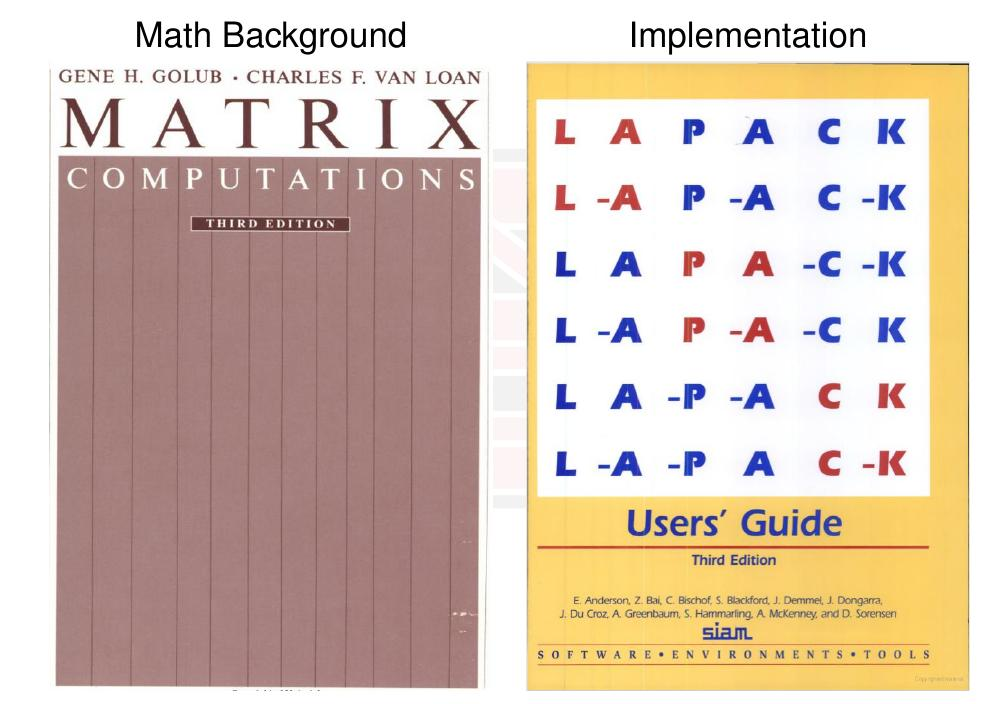
\includegraphics[width=.7\textwidth,height=.7\textheight]{lapack.jpeg}
%\caption{English Dartboard}
\label{fig1.eps}
\end{figure} 
\end{frame}
%%%%%%%%%%%%%%%%%%%%%%%%%%%%%%%%%%%%%%%%%%%%%%%%%%%%%%
%%%%%%%%%%%%%%%%%%%%%%%%%%%%%%%%%%%%%%%%%%%%%%%%%%%%%
\subsection{ }
\begin{frame}[fragile]{Hierarchy Libraries}
\begin{figure}[htp]
\centering
%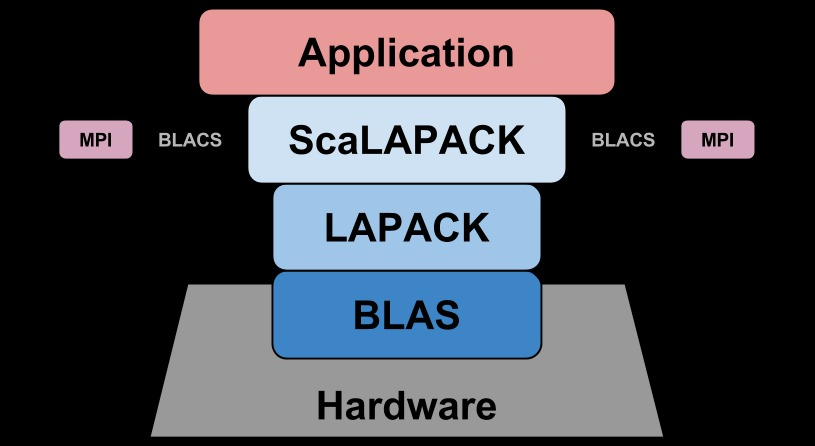
\includegraphics[width=.7\textwidth,height=.7\textheight]{LAPACK_Stack.jpg}
%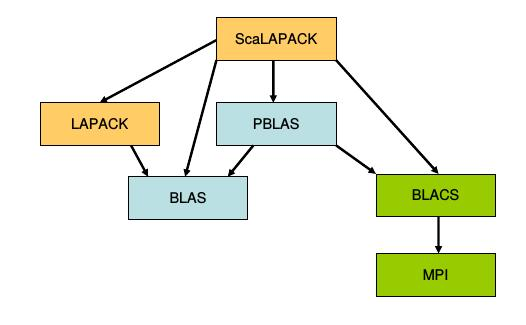
\includegraphics[width=.7\textwidth,height=.7\textheight]{Lapack_2.jpeg}
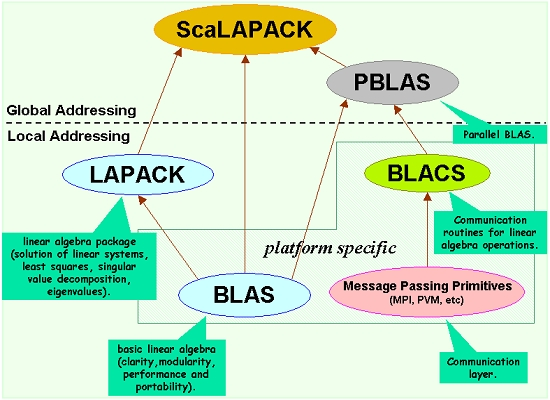
\includegraphics[width=.7\textwidth,height=.7\textheight]{components.jpg}
%\caption{English Dartboard}
\label{fig1.eps}
\end{figure} 
\end{frame}

%%%%%%%%%%%%%%%%%%%%%%%%%%%%%%%%%%%%%%%%%%%%%%%%%%%%%%
%%%%%%%%%%%%%%%%%%%%%%%%%%%%%%%%%%%%%%%%%%%%%%%%%%%%%
\section{\scshape Examples:  Exponential Matrix}
\begin{frame}[fragile]{Example : Exponential Matrix}
\begin{huge}\begin{equation*}
 y=\rm{e}^{A}
\end{equation*}\end{huge}


\begin{description}
\item [Example 1:] A is Symmetric, then all of its eigenvalue are real
\item [Example 2:] A is Real, then eigenvalue are complex
\end{description}
\end{frame}
%%%%%%%%%%%%%%%%%%%%%%%%%%%%%%%%%%%%%%%%%%%%%%%%%%%%%%
%%%%%%%%%%%%%%%%%%%%%%%%%%%%%%%%%%%%%%%%%%%%%%%%%%%%%%
\section{}
\begin{frame}{Exponential Matrix}
\begin{small}Consider the Taylor series of exponential 
\begin{equation*}
 \mathrm{e}^x = \displaystyle\sum_{k=0}^{\infty}\frac{x^k}{k!}  =  1 + x + \frac{x^2}{2!} +\frac{x^2}{3!} + \cdots + \frac{x^p}{p!}+\cdots
\end{equation*}
given a square matrix A we can define the matrix exponential as follows
\begin{equation*}
 \mathrm{e}^A = \displaystyle\sum_{k=0}^{\infty}\frac{A^k }{k!} =  I + A + \frac{A^2}{2!} +\frac{A^2}{3!} + \cdots + \frac{A^p}{p!}+\cdots
\end{equation*}\end{small}         
\end{frame}
%%%%%%%%%%%%%%%%%%%%%%%%%%%%%%%%%%%%%%%%%%%%%%%%%%%%%%
%%%%%%%%%%%%%%%%%%%%%%%%%%%%%%%%%%%%%%%%%%%%%%%%%%%%%%
\subsection{\scshape Symmetric Matrix}
\begin{frame}{Symmetric Matrix}
\begin{tiny}Let be $A ∈\in \mathbb{R}^{n\times n}$ symmetric $A = A^T$, then the matrix has a complete set of linear independent eigenvectors $v_1, v_2,\cdots,v_n$
\begin{equation*}
A\;v_k = \lambda_k v_k,\hspace{1cm} k = 1,2,\cdots,n
\end{equation*}
Thus, defining the matrix $T = [v_1, v_2,\cdots,v_n]$ whose columns are the eigenvectors we have
\begin{equation*}
 AT = [A\;v_1, A\;v_2,\cdots, A\;v_n ] = [\lambda_1 v_1, \lambda_2 v_2 ,\cdots, \lambda_n v_n ] = T \Lambda
\end{equation*}
and thus $A = T \Lambda T^{-1}$ where
\[\Lambda = \left( \begin{array}{cccc}
\lambda_1 &           &  & \\
          & \lambda_2 &  & \\
          &           & \ddots & \\          
          &           &  & \lambda_n \end{array} \right)\] 
Using $A = T \Lambda T^{-1}$ we can write     
\begin{equation*}
 \mathrm{e}^A = \displaystyle\sum_{k=0}^{\infty}\frac{1}{k!} A^k =  T \left(\displaystyle\sum_{k=0}^{\infty}\frac{1}{k!} \Lambda^k\right) T^{-1} = T\mathrm{e}^{\Lambda}T^{-1}
\end{equation*}
\[\mathrm{e}^A = T \left(\begin{array}{cccc}
\mathrm{e}^\lambda_1 &           &  & \\
          & \mathrm{e}^\lambda_2 &  & \\
          &           & \ddots & \\          
          &           &  & \mathrm{e}^\lambda_n \end{array} \right) T^{-1}\]
\end{tiny} 
\end{frame}
%%%%%%%%%%%%%%%%%%%%%%%%%%%%%%%%%%%%%%%%%%%%%%%%%%%%%%
%%%%%%%%%%%%%%%%%%%%%%%%%%%%%%%%%%%%%%%%%%%%%%%%%%%%%%
\subsection{}
\begin{frame}[fragile]{Symmetric Matrix - Solve with Matlab}
\begin{minipage}{.3\textwidth} 
\pause
\begin{tiny}
\begin{verbatim}
>> A = [5 4; 4 5]
A =

   4   5
   5   4
   
>> expm(A)
ans =

   4052.9   4050.2
   4050.2   4052.9 

>> [v lambda]=eig(A)
v =

  -0.70711   0.70711
   0.70711   0.70711

lambda =

   1   0
   0   9

>> v*expm(lambda)*inv(v)
ans =

   4052.9   4050.2
   4050.2   4052.9
\end{verbatim}
\end{tiny} 
\end{minipage}
\begin{minipage}{.65\textwidth} %
\pause
\begin{tiny}
\begin{verbatim}
>>  A = [ 1.96   -6.49  -0.47   -7.20   -0.65;
          -6.49    3.80  -6.39    1.50   -6.34;
          -0.47   -6.39   4.17   -1.51    2.67;
          -7.20    1.50  -1.51    5.70    1.80;
          -0.65   -6.34   2.67    1.80   -7.10; ]
A =

   1.96000  -6.49000  -0.47000  -7.20000  -0.65000
  -6.49000   3.80000  -6.39000   1.50000  -6.34000
  -0.47000  -6.39000   4.17000  -1.51000   2.67000
  -7.20000   1.50000  -1.51000   5.70000   1.80000
  -0.65000  -6.34000   2.67000   1.80000  -7.10000
  
>> expm(A)

ans =

   2.3433e+06  -2.8945e+06   1.9081e+06  -2.1849e+06   7.7534e+05
  -2.8945e+06   3.5800e+06  -2.3616e+06   2.6972e+06  -9.6022e+05
   1.9081e+06  -2.3616e+06   1.5583e+06  -1.7775e+06   6.3382e+05
  -2.1849e+06   2.6972e+06  -1.7775e+06   2.0376e+06  -7.2207e+05
   7.7534e+05  -9.6022e+05   6.3382e+05  -7.2207e+05   2.5787e+05
\end{verbatim}
\end{tiny}
\end{minipage}
\end{frame}
%%%%%%%%%%%%%%%%%%%%%%%%%%%%%%%%%%%%%%%%%%%%%%%%%%%%%
%%%%%%%%%%%%%%%%%%%%%%%%%%%%%%%%%%%%%%%%%%%%%%%%%%%%%%
\subsection{}
\begin{frame}[fragile]{Symmetric Matrix - Solve with C}
\begin{scriptsize}
\begin{itemize}
 \item Allocate memory space for the input/output parameters and workspace arrays, $A$ must be real symmetric matrix  (* require memory allocation -  malloc).
 \[*A, *B, *W, *Z, *WORK, *ISUPPZ, *IWORK \]
 \item Compute the eigenvalues and eigenvectors of $A$. 
 \[(W, Z)\]
 Setup Lapack library \textbf{dsyevr}
\begin{tiny}\verb+dsyevr('V', 'A', 'L', N, A, N, 0, 0 0, 0, dlamch('S'), &M, W, Z, N, ISUPPZ,+\end{tiny}
\begin{tiny}\verb+        WORK, 26*N, IWORK, 10*N);+\end{tiny}
 \item Allocate and initialise matrix $B = Z*D$. 
 \item Compute \[D = exp(W_j)\]
 \item Compute  $B = Z*D$
 \item Compute the product, using Cblas library \textbf{cblas\_dgemm} \[A = B*Z^T \]  
\begin{tiny} \verb+cblas_dgemm(CblasColMajor, CblasNoTrans, CblasTrans, N, N, N, 1, B, N, Z, N, 0, A, N)+\end{tiny}
 \item Print results $C = expm(A) = Z*D*Z^T $
\end{itemize}\end{scriptsize}
\end{frame}
%%%%%%%%%%%%%%%%%%%%%%%%%%%%%%%%%%%%%%%%%%%%%%%%%%%%%%
%%%%%%%%%%%%%%%%%%%%%%%%%%%%%%%%%%%%%%%%%%%%%%%%%%%%%%
\subsection{}
\begin{frame}[fragile]{Symmetric Matrix - C interface}
\begin{tiny}
%Lapack library computes the eigenvalues and eigenvectors of a real symmetric matrix
LAPACK C wrapper, link your program with the \verb+lapack_wrapper.a+ library in the lib directory. 
\begin{verbatim}
static int dsyevr(char JOBZ, char RANGE, char UPLO, int N, double *A, int LDA, double VL,
                  double VU,int IL, int IU, double ABSTOL, int *M, double *W, double *Z,
                  int LDZ, int *ISUPPZ, double *WORK, int LWORK, int *IWORK, int LIWORK) {
             
  extern void dsyevr_(char *JOBZp,char *RANGEp, char *UPLOp, int *Np, double *A, int *LDAp,
                     double *VLp, double *VUp, int *ILp, int *IUp, double *ABSTOLp, int *Mp,
                     double *W, double *Z, int *LDZp, int *ISUPPZ,double *WORK, int *LWORKp,
                     int *IWORK, int *LIWORKp, int *INFOp);
 
            int INFO;
       
            dsyevr_(&JOBZ, &RANGE, &UPLO, &N, A, &LDA, &VL, &VU, &IL, &IU, &ABSTOL, M, W,
                    Z, &LDZ, ISUPPZ, WORK, &LWORK, IWORK, &LIWORK, &INFO);
	    
            return INFO;
}

static double dlamch(char CMACH) {
      extern double dlamch_(char *CMACHp);
      return dlamch_(&CMACH);
 }            
\end{verbatim}
\end{tiny} 
\end{frame}
%%%%%%%%%%%%%%%%%%%%%%%%%%%%%%%%%%%%%%%%%%%%%%%%%%%%%%
%%%%%%%%%%%%%%%%%%%%%%%%%%%%%%%%%%%%%%%%%%%%%%%%%%%%%%
\subsection{}
\begin{frame}[fragile]{LAPACK - DSYEVR}
\begin{tiny}\verb+dsyevr('V', 'A', 'L', N, A, N, 0, 0 0, 0, dlamch('S'), &M, W, Z, N, ISUPPZ, WORK, 26*N,+\end{tiny}
\begin{tiny}\verb+       IWORK, 10*N);+\end{tiny}
\begin{tiny}
\begin{verbatim}
subroutine dsyevr(  
		    character                            JOBZ,
		    character                            RANGE,
		    character                            UPLO,
		    integer                              N,
		    double precision, dimension(lda,*)   A,
		    integer                              LDA,
		    double precision                     VL,
		    double precision                     VU,
		    integer                              IL,
		    integer                              IU,
		    double precision                     ABSTOL,
		    integer                              M,
		    double precision, dimension(*)       W,
		    double precision, dimension(ldz,*)   Z,
		    integer                              LDZ,
		    integer, dimension(*)                ISUPPZ,
		    double precision, dimension(*)       WORK,
		    integer                              LWORK,
		    integer, dimension(*)                IWORK,
		    integer                              LIWORK,
		    integer                              INFO 
)	         
\end{verbatim}
\end{tiny} 
\href{http://www.netlib.org/lapack/explore-html/d2/d8a/group__double_s_yeigen_ga2ad9f4a91cddbf67fe41b621bd158f5c.html#ga2ad9f4a91cddbf67fe41b621bd158f5c}{LAPACK- DSYEVR}
\end{frame}
%%%%%%%%%%%%%%%%%%%%%%%%%%%%%%%%%%%%%%%%%%%%%%%%%%%%%%
%%%%%%%%%%%%%%%%%%%%%%%%%%%%%%%%%%%%%%%%%%%%%%%%%%%%%%
\subsection{}
\begin{frame}[fragile]{BLAS - DGEMM}
\[C := \alpha* A * B + \beta * C\]
\begin{tiny} \verb+cblas_dgemm(CblasColMajor, CblasNoTrans, CblasTrans, N, N, N, 1, B, N, Z, N, 0, A, N)+\end{tiny}
\begin{tiny}
\begin{verbatim}
subroutine dgemm (
	  character                                 TRANSA,
	  character                                 TRANSB,
	  integer                                   M,
	  integer                                   N,
	  integer                                   K,
	  double precision                          ALPHA,
	  double precision, dimension(lda,*)        A,
	  integer                                   LDA,
	  double precision, dimension(ldb,*)        B,
	  integer                                   LDB,
	  double precision                          BETA,
	  double precision, dimension(ldc,*)        C,
	  integer                                   LDC 
)
\end{verbatim}
\end{tiny} 
\href{https://software.intel.com/en-us/node/520775}{BLAS - DGEMM}
\end{frame}
%%%%%%%%%%%%%%%%%%%%%%%%%%%%%%%%%%%%%%%%%%%%%%%%%%%%%%
%%%%%%%%%%%%%%%%%%%%%%%%%%%%%%%%%%%%%%%%%%%%%%%%%%%%%%
\subsection{}
\begin{frame}[fragile]{Real Matrix - Solve with Matlab}
\begin{tiny}
\begin{verbatim}
>> A = [-1.01   0.86  -4.60   3.31  -4.81;
         3.98   0.53  -7.04   5.29   3.55;
         3.30   8.26  -3.89   8.20  -1.51;
         4.43   4.96  -7.66  -7.33   6.18;
         7.31  -6.43  -6.16   2.47   5.58]

>> [V l] = eig(A)
V =

   0.10806 + 0.16865i   0.10806 - 0.16865i   0.73223 + 0.00000i   0.73223 - 0.00000i   0.46065 + 0.00000i
   0.40631 - 0.25901i   0.40631 + 0.25901i  -0.02646 - 0.01695i  -0.02646 + 0.01695i   0.33770 + 0.00000i
   0.10236 - 0.50880i   0.10236 + 0.50880i   0.19165 - 0.29257i   0.19165 + 0.29257i   0.30874 + 0.00000i
   0.39863 - 0.09133i   0.39863 + 0.09133i  -0.07901 - 0.07808i  -0.07901 + 0.07808i  -0.74385 + 0.00000i
   0.53954 + 0.00000i   0.53954 - 0.00000i  -0.29160 - 0.49310i  -0.29160 + 0.49310i   0.15853 + 0.00000i

l =
    2.85813 + 10.76275i                      0                      0                      0                      0
                      0    2.85813 - 10.76275i                      0                      0                      0
                      0                      0   -0.68667 +  4.70426i                      0                      0
                      0                      0                      0   -0.68667 -  4.70426i                      0
                      0                      0                      0                      0  -10.46292 +  0.00000i
\end{verbatim}
\end{tiny} 
\end{frame}
%%%%%%%%%%%%%%%%%%%%%%%%%%%%%%%%%%%%%%%%%%%%%%%%%%%%%%
%%%%%%%%%%%%%%%%%%%%%%%%%%%%%%%%%%%%%%%%%%%%%%%%%%%%%%
\subsection{}
\begin{frame}[fragile]{Real Matrix - Solve with Matlab}
\begin{tiny}
\begin{verbatim}
>> B=V*expm(l)
B =

   2.42549 - 2.51083i   2.42549 + 2.51083i  -0.00299 - 0.36848i  -0.00299 + 0.36848i   0.00001 + 0.00000i
  -6.02638 - 5.84897i  -6.02638 + 5.84897i  -0.00842 + 0.01339i  -0.00842 - 0.01339i   0.00001 + 0.00000i
  -9.04024 + 0.31021i  -9.04024 - 0.31021i  -0.14801 - 0.09525i  -0.14801 + 0.09525i   0.00001 + 0.00000i
  -3.15192 - 6.39298i  -3.15192 + 6.39298i  -0.03897 + 0.04008i  -0.03897 - 0.04008i  -0.00002 + 0.00000i
  -2.16965 - 9.14981i  -2.16965 + 9.14981i  -0.24695 + 0.14876i  -0.24695 - 0.14876i   0.00000 + 0.00000i

>> C =B*inv(V)
C =

   -0.50217 +  0.00000i    4.56041 +  0.00000i    2.01829 +  0.00000i    2.38722 +  0.00000i   -0.98493 +  0.00000i
   -6.36228 +  0.00000i   -4.83109 +  0.00000i   12.28998 +  0.00000i   -2.47319 +  0.00000i   -6.76137 +  0.00000i
   -3.85152 -  0.00000i  -13.76345 -  0.00000i    6.27992 -  0.00000i   -6.46124 +  0.00000i   -2.03676 +  0.00000i
   -5.50963 +  0.00000i   -0.11275 +  0.00000i   10.85609 +  0.00000i   -0.33509 +  0.00000i   -6.46545 +  0.00000i
   -7.10558 +  0.00000i    3.60664 +  0.00000i   13.60548 +  0.00000i    1.03809 +  0.00000i   -8.66237 +  0.00000i

>> expm(A)
ans =

   -0.50217    4.56041    2.01829    2.38722   -0.98493
   -6.36228   -4.83109   12.28998   -2.47319   -6.76137
   -3.85152  -13.76345    6.27992   -6.46124   -2.03676
   -5.50963   -0.11275   10.85609   -0.33509   -6.46545
   -7.10558    3.60664   13.60548    1.03809   -8.66237
\end{verbatim}
\end{tiny}
\end{frame}
%%%%%%%%%%%%%%%%%%%%%%%%%%%%%%%%%%%%%%%%%%%%%%%%%%%%%%
%%%%%%%%%%%%%%%%%%%%%%%%%%%%%%%%%%%%%%%%%%%%%%%%%%%%%%
\subsection{\scshape Real Matrix}
\begin{frame}{Real Matrix}
\begin{tiny}
Let be $A ∈\in \mathbb{R}^{n\times n}$, then the matrix exponential can be computed starting from Jordan normal form (or Jordan canonical form).

Theorem (Jordan normal form) Any square matrix $A ∈\in \mathbb{R}^{n\times n}$, is similar to a block diagonal matrix $J$ , i.e. $T^{-1} AT = J$ where
\[J = \left( \begin{array}{cccc}
J_1 &           &  & \\
          & J_2 &  & \\
          &           & \ddots & \\          
          &           &  & J_m \end{array} \right) 
\hspace{.5cm}\mbox{and}\hspace{.5cm}
J_k = \left( \begin{array}{cccc}
\lambda_k &    1      &  &      \\
          & \lambda_k & \ddots & \\
          &           & \ddots & 1\\          
          &           &  & \lambda_k \end{array} \right) = \lambda_k I + N
% \lambda_k \; \left( \begin{array}{cccc}
%    1       &          &         &      \\
%           & 1         & \ddots  &   \\
%           &           &  \ddots & \\          
%           &           &         & 1\end{array} \right)  + 
% \left( \begin{array}{cccc}
%      0    &    1  &        &      \\
%           &   0   & \ddots & \\
%           &       & \ddots & 1\\          
%           &       &        & 0 \end{array} \right)          
          \] 
          
The column of $T = [t_{1,1} , t_{1,2} , . . . , t_{m,n_m} , t_{m,n_{m-1}}]$ are generalized eigenvectors, i.e.

\[At_{k,j} = \left\{ \begin{array}{lcc}
\lambda_k t_{k,j}            &    \mbox{if}  & j=1  \\
\lambda_k t_{k,j} +t_{k,j-1} &    \mbox{if}  & j>1  \end{array} \right.\] 

\[\mathrm{e}^A = \displaystyle\sum_{k=0}^{\infty}\frac{1}{k!} A^k =  \displaystyle\sum_{k=0}^{\infty}\frac{1}{k!} \left(T\;\Lambda^k\; T^{-1}\right)^k 
= T \left(\begin{array}{cccc}
\mathrm{e}^{J_1} &           &  & \\
          & \mathrm{e}^{J_2} &  & \\
          &           & \ddots & \\          
          &           &  & \mathrm{e}^{J_m} \end{array} \right) T^{-1}\]   
          
\end{tiny} 
          
\end{frame}
%%%%%%%%%%%%%%%%%%%%%%%%%%%%%%%%%%%%%%%%%%%%%%%%%%%%%
%%%%%%%%%%%%%%%%%%%%%%%%%%%%%%%%%%%%%%%%%%%%%%%%%%%%%%
\subsection{}
\begin{frame}[fragile]{Code description implementation}
\begin{scriptsize}
\begin{itemize}
 \item Allocate memory space for the input/output parameters and workspace arrays, $A$ must be real (* require memory allocation -  malloc).
 \[*A, *WR, *WI, *VL, *VR,  *WORK \] 
 \item Compute the eigenvalues $(WR, WI)$ and left and right eigenvectors $(VL, VR)$
 \[(WR,WI,VL,VR)\]
 Setup Lapack library \textbf{dgeev}
 \verb+dgeev('V', 'V', N, A, N, WR, WI, VL, N, VR, N, WORK, 4*N); + 
 \item Allocate memory for $(\exp(WR), \exp(WI))$ and  compute \[D = exp(WR + I*WI)\]
 \item Allocate memory for $B = VR*D$ and  compute  \[B = VR*D\]
 \item Find the inverse matrix of $VR^{-1}$
 \item Compute the product $B*VR^{-1}$, using Cblas library \textbf{cblas\_zgemm}
 \[C =  \alpha*A*B + \beta*C = 1*B*invVR + 0*C*\]
\begin{tiny}\verb+cblas_zgemm(CblasColMajor, CblasNoTrans, CblasNoTrans, m, n, k, &alpha, B, LDA,+ \end{tiny}
\begin{tiny}\verb+            invVR, LDB, &beta, C, LDC);+ \end{tiny}
 \item Print results $C = expm(A) = B*VR^{-1} = VR*D*VR^{-1}$
\end{itemize}\end{scriptsize}
\end{frame}
%%%%%%%%%%%%%%%%%%%%%%%%%%%%%%%%%%%%%%%%%%%%%%%%%%%%%
%%%%%%%%%%%%%%%%%%%%%%%%%%%%%%%%%%%%%%%%%%%%%%%%%%%%%%
\subsection{}
\begin{frame}[fragile]{Code description implementation}
\begin{scriptsize}
 Find the inverse matrix of $VR^{-1}$
\begin{itemize}
  \item Allocate memory space for
   \[*IPIV,  *WORK \] 
  \item LU factorization 
  \begin{verbatim}
       zgetrf_(&N, &N, A, &N, IPIV, &INFO);
  \end{verbatim}
\item Inverse 
  \begin{verbatim}
       zgetri_(&N, A, &N, IPIV, WORK, &LWORK, &INFO);
  \end{verbatim}
   \item Print results $VR^{-1}$
\end{itemize}\end{scriptsize}
\end{frame}
%%%%%%%%%%%%%%%%%%%%%%%%%%%%%%%%%%%%%%%%%%%%%%%%%%%%%%
%%%%%%%%%%%%%%%%%%%%%%%%%%%%%%%%%%%%%%%%%%%%%%%%%%%%%%
\subsection{}
\begin{frame}[fragile]{Real Matrix - C interface}
\begin{tiny}
%Lapack library computes the eigenvalues and eigenvectors of a real symmetric matrix
LAPACK C wrapper, link your program with the \verb+lapack_wrapper.a+ library in the lib directory. 
\begin{verbatim}
static int dgeev( char JOBVL, char JOBVR, int N, double *A, int LDA, double *WR, double *WI,
                 double *VL, int LDVL, double *VR, int LDVR, double *WORK, int LWORK){

   extern void dgeev_( char *JOBVLp, char *JOBVRp, int *Np, double *A, int *LDAp, 
                       double *WR, double *WI, double *VL, int *LDVLp, double *VR, 
                       int *LDVRp, double *WORK,int *LWORKp, int *INFOp );

   int INFO;

   dgeev_(&JOBVL, &JOBVR, &N, A, &LDA, WR, WI, VL, &LDVL, VR, &LDVR, WORK, &LWORK, &INFO);

   return INFO;
}
\end{verbatim}
Generate LU decomposition of a general matrix
\begin{verbatim}
extern void zgetrf_(int* M, int *N, double complex* A, int* lda, int* IPIV, int* INFO);
\end{verbatim}
Generate the inverse matrix given a LU decomposition of the matrix
\begin{verbatim}
extern void zgetri_(int* N, double complex* A, int* lda, int* IPIV, double complex* WORK, 
                    int* lwork, int* INFO);
\end{verbatim}
Use BLAS library  $C =  \alpha*A*B + \beta*C = 1*B*invVR + 0*C$
\begin{verbatim}
cblas_zgemm(CblasColMajor, CblasNoTrans, CblasNoTrans, m, n, k, &alpha, BB, LDA, invVR,
            LDB, &beta, C, LDC);
\end{verbatim}
\end{tiny}
\end{frame}

% %%%%%%%%%%%%%%%%%%%%%%%%%%%%%%%%%%%%%%%%%%%%%%%%%%%%%
% %%%%%%%%%%%%%%%%%%%%%%%%%%%%%%%%%%%%%%%%%%%%%%%%%%%%%%
% \section{\scshape Implement Code 2}
% \begin{frame}{Working on a complex matrix}
% 
% \end{frame}
% %%%%%%%%%%%%%%%%%%%%%%%%%%%%%%%%%%%%%%%%%%%%%%%%%%%%%
% %%%%%%%%%%%%%%%%%%%%%%%%%%%%%%%%%%%%%%%%%%%%%%%%%%%%%%
% \section{\scshape Implement Code 2}
% \begin{frame}{Working on a complex matrix}
% 
% \end{frame}
% %%%%%%%%%%%%%%%%%%%%%%%%%%%%%%%%%%%%%%%%%%%%%%%%%%%%%
% %%%%%%%%%%%%%%%%%%%%%%%%%%%%%%%%%%%%%%%%%%%%%%%%%%%%%%
% 
% %%%%%%%%%%%%%%%%%%%%%%%%%%%%%%%%%%%%%%%%%%%%%%%%%%%%%%
% %%%%%%%%%%%%%%%%%%%%%%%%%%%%%%%%%%%%%%%%%%%%%%%%%%%%%%
% \section{\scshape Implement Code 2}
% \begin{frame}{Working on a complex matrix}
% 
% \end{frame}
%%%%%%%%%%%%%%%%%%%%%%%%%%%%%%%%%%%%%%%%%%%%%%%%%%%%%
%%%%%%%%%%%%%%%%%%%%%%%%%%%%%%%%%%%%%%%%%%%%%%%%%%%%%%
\section{\scshape Linking to others Web Pages}
\begin{frame}[fragile]{For further references see :}
\begin{scriptsize}
%For further references see :% \href{http://www.sharelatex.com}{Something Linky} or go to the next url: \url{http://www.sharelatex.com}
\begin{itemize}
\item \href{http://physics.oregonstate.edu/~landaur/nacphy/lapack/fortran.html}{Using Lapack Routines in Fortran Programs}
\item \href{http://physics.oregonstate.edu/~landaur/nacphy/lapack/cprogp.html}{Using Lapack Routines in C Programs}
\item \href{https://people.sc.fsu.edu/~jburkardt/f_src/lapack_examples/lapack_examples.html}{LAPACK EXAMPLES - Example Programs for LAPACK}
\item \href{http://www.netlib.org/lapack/explore-html/dir_01b0e9dedaacaaad221a964f5affeb80.html}{LAPACK: Linear Algebra PACKage}
\item \href{http://www.netlib.org/lapack/}{Linear Algebra PACKage}
\item \href{http://www.netlib.org/lapack/lapacke.html}{The LAPACKE C Interface to LAPACK}
\item \href{https://software.intel.com/en-us/node/528727}{Calling LAPACK, BLAS, and CBLAS Routines from C/C++ Language Environments}
\item \href{http://www.netlib.org/lapack/explore-html/d5/df8/example___d_g_e_s_v__colmajor_8c.html}{example\_DGESV\_colmajor.c File Reference}
\item \href{http://www.netlib.org/lapack/explore-html/d6/d06/example___d_g_e_s_v__rowmajor_8c_source.html}{example\_DGESV\_rowmajor.c}
\item \href{https://userinfo.surfsara.nl/systems/lisa/software/lapacke}{Using LAPACK from C}
\item \href{https://software.intel.com/en-us/articles/intel-math-kernel-library-documentation}{Intel® Math Kernel Library – Documentation}
\item \href{https://en.wikipedia.org/wiki/Math_Kernel_Library}{Math Kernel Library}
\item \href{http://www.seehuhn.de/pages/matrixfn}{Calculating the Square Root of a Matrix}
\item \href{http://courses.washington.edu/css342/zander/css332/passby.html}{Function pass by value vs. pass by reference}
\item \href{https://www.codingunit.com/c-tutorial-call-by-value-or-call-by-reference}{C Tutorial – Call by Value or Call by Reference}
\item \href{https://gcc.gnu.org/onlinedocs/gcc-4.9.2/gfortran/Argument-passing-conventions.html}{Argument passing conventions}
\item \href{http://www.netlib.org/lapack/explore-html/d2/d8a/group__double_s_yeigen_ga2ad9f4a91cddbf67fe41b621bd158f5c.html#ga2ad9f4a91cddbf67fe41b621bd158f5c}{LAPACK- DSYEVR}
\item \href{https://software.intel.com/sites/products/documentation/doclib/mkl_sa/11/mkl_lapack_examples/dsyevr.htm}{DSYEVR Example}
\item \href{http://www.netlib.org/lapack/lapwrapc/}{C wrapper for LAPACK}
\item \href{http://www.netlib.org/lapack/explore-html/d1/d54/group__double__blas__level3_gaeda3cbd99c8fb834a60a6412878226e1.html#gaeda3cbd99c8fb834a60a6412878226e1}{BLAS - DGEMM}
\item \href{https://www.christophlassner.de/using-blas-from-c-with-row-major-data.html}{Using BLAS from C with row major data}
\item \href{https://software.intel.com/en-us/node/520775}{cblas\_?gemm}
\end{itemize}
\end{scriptsize}
\end{frame}
%%%%%%%%%%%%%%%%%%%%%%%%%%%%%%%%%%%%%%%%%%%%%%%%%%%%%
%%%%%%%%%%%%%%%%%%%%%%%%%%%%%%%%%%%%%%%%%%%%%%%%%%%%%%
\section{END}
\begin{frame}{END}
  \begin{center}
  \Large\textbf{QUESTIONS ???}
  \end{center}
\end{frame}
\end{document}